% ========================================
%	Header einbinden
% ========================================

\documentclass[bibtotoc,titlepage]{scrartcl}

% Deutsche Spracheinstellungen
\usepackage[ngerman,german]{babel, varioref}
\usepackage[T1]{fontenc}
\usepackage[utf8]{inputenc}

%\usepackage{marvosym}

\usepackage{amsfonts}
\usepackage{amssymb}
\usepackage{amsmath}
\usepackage{amscd}
\usepackage{amstext}

\usepackage{longtable}

%\usepackage{bibgerm}

\usepackage{footnpag}

\usepackage{ifthen}                 %%% package for conditionals in TeX
\usepackage[amssymb]{SIunits}
%Für textumflossene Bilder und Tablellen
%\usepackage{floatflt} - veraltet

%Für Testzwecke aktivieren, zeigt labels und refs im Text an.
%\usepackage{showkeys}

% Abstand zwischen zwei Absätzen nach DIN (1,5 Zeilen)
% \setlength{\parskip}{1.5ex plus0.5ex minus0.5ex}

% Einrückung am Anfang eines neuen Absatzes nach DIN (keine)
%\setlength{\parindent}{0pt}

% Ränder definieren
% \setlength{\oddsidemargin}{0.3cm}
% \setlength{\textwidth}{15.6cm}

% bessere Bildunterschriften
%\usepackage[center]{caption2}


% Problemlösungen beim Umgang mit Gleitumgebungen
\usepackage{float}

% Nummeriert bis zur Strukturstufe 3 (also <section>, <subsection> und <subsubsection>)
%\setcounter{secnumdepth}{3}

% Führt das Inhaltsverzeichnis bis zur Strukturstufe 3
%\setcounter{tocdepth}{3}
\usepackage[version=3]{mhchem}
	\mhchemoptions{minus-sidebearing-left=0.06em, minus-sidebearing-right=0.11em}
\usepackage{exscale}

\newenvironment{dsm} {\begin{displaymath}} {\end{displaymath}}
\newenvironment{vars} {\begin{center}\scriptsize} {\normalsize \end{center}}


\newcommand {\en} {\varepsilon_0}               % Epsilon-Null aus der Elektrodynamik
\newcommand {\lap} {\; \mathbf{\Delta}}         % Laplace-Operator
\newcommand {\R} { \mathbb{R} }                 % Menge der reellen Zahlen
\newcommand {\e} { \ \mathbf{e} }               % Eulersche Zahl
\renewcommand {\i} { \mathbf{i} }               % komplexe Zahl i
\newcommand {\N} { \mathbb{N} }                 % Menge der nat. Zahlen
\newcommand {\C} { \mathbb{C} }                 % Menge der kompl. Zahlen
\newcommand {\Z} { \mathbb{Z} }                 % Menge der kompl. Zahlen
\newcommand {\limi}[1]{\lim_{#1 \rightarrow \infty}} % Limes unendlich
\newcommand {\sumi}[1]{\sum_{#1=0}^\infty}
\newcommand {\rot} {\; \mathrm{rot} \,}         % Rotation
\newcommand {\grad} {\; \mathrm{grad} \,}       % Gradient
\newcommand {\dive} {\; \mathrm{div} \,}        % Divergenz
\newcommand {\dx} {\; \mathrm{d} }              % Differential d
\newcommand {\cotanh} {\; \mathrm{cotanh} \,}   %Cotangenshyperbolicus
\newcommand {\asinh} {\; \mathrm{areasinh} \,}  %Area-Sinus-Hyp.
\newcommand {\acosh} {\; \mathrm{areacosh} \,}  %Area-Cosinus-H.
\newcommand {\atanh} {\; \mathrm{areatanh} \,}  %Area Tangens-H.
\newcommand {\acoth} {\; \mathrm{areacoth} \,}  % Area-cotangens
\newcommand {\Sp} {\; \mathrm{Sp} \,}
\newcommand {\mbe} {\stackrel{\text{!}}{=}}     %Must Be Equal
\newcommand{\qed} { \hfill $\square$\\}
\renewcommand{\i} {\imath}
\def\captionsngerman{\def\figurename{\textbf{Abb.}}}

%%%%%%%%%%%%%%%%%%%%%%%%%%%%%%%%%%%%%%%%%%%%%%%%%%%%%%%%%%%%%%%%%%%%%%%%%%%%
% SWITCH FOR PDFLATEX or LATEX
%%%%%%%%%%%%%%%%%%%%%%%%%%%%%%%%%%%%%%%%%%%%%%%%%%%%%%%%%%%%%%%%%%%%%%%%%%%%
%%%
\ifx\pdfoutput\undefined %%%%%%%%%%%%%%%%%%%%%%%%%%%%%%%%%%%%%%%%% LATEX %%%
%%%
\usepackage[dvips]{graphicx}       %%% graphics for dvips
\DeclareGraphicsExtensions{.eps,.ps}   %%% standard extension for included graphics
\usepackage[ps2pdf]{thumbpdf}      %%% thumbnails for ps2pdf
\usepackage[ps2pdf,                %%% hyper-references for ps2pdf
bookmarks=true,%                   %%% generate bookmarks ...
bookmarksnumbered=true,%           %%% ... with numbers
hypertexnames=false,%              %%% needed for correct links to figures !!!
breaklinks=true,%                  %%% breaks lines, but links are very small
linkbordercolor={0 0 1},%          %%% blue frames around links
pdfborder={0 0 112.0}]{hyperref}%  %%% border-width of frames
%                                      will be multiplied with 0.009 by ps2pdf
%
\hypersetup{ pdfauthor   = {Hannes Franke; Julius Tilly},
pdftitle    = {V301 Innenwiderstand und Leistungsanpassung}, pdfsubject  = {Protokoll FP}, pdfkeywords = {V301, Innenwiderstand, Leistungsanpassung},
pdfcreator  = {LaTeX with hyperref package}, pdfproducer = {dvips
+ ps2pdf} }
%%%
\else %%%%%%%%%%%%%%%%%%%%%%%%%%%%%%%%%%%%%%%%%%%%%%%%%%%%%%%%%% PDFLATEX %%%
%%%
\usepackage[pdftex]{graphicx}      %%% graphics for pdfLaTeX
\DeclareGraphicsExtensions{.pdf}   %%% standard extension for included graphics
\usepackage[pdftex]{thumbpdf}      %%% thumbnails for pdflatex
\usepackage[pdftex,                %%% hyper-references for pdflatex
bookmarks=true,%                   %%% generate bookmarks ...
bookmarksnumbered=true,%           %%% ... with numbers
hypertexnames=false,%              %%% needed for correct links to figures !!!
breaklinks=true,%                  %%% break links if exceeding a single line
linkbordercolor={0 0 1},
linktocpage]{hyperref} %%% blue frames around links
%                                  %%% pdfborder={0 0 1} is the default
\hypersetup{
pdftitle    = {V301 Innenwiderstand und Leistungsanpassung}, 
pdfsubject  = {Protokoll AP}, 
pdfkeywords = {V301, Innenwiderstand, Leistungsanpassung},
pdfsubject  = {Protokoll AP},
pdfkeywords = {V301, Innenwiderstand, Leistungsanpassung}}
%                                  %%% pdfcreator, pdfproducer,
%                                      and CreationDate are automatically set
%                                      by pdflatex !!!
\pdfadjustspacing=1                %%% force LaTeX-like character spacing
\usepackage{epstopdf}
%
\fi %%%%%%%%%%%%%%%%%%%%%%%%%%%%%%%%%%%%%%%%%%%%%%%%%%% END OF CONDITION %%%
%%%%%%%%%%%%%%%%%%%%%%%%%%%%%%%%%%%%%%%%%%%%%%%%%%%%%%%%%%%%%%%%%%%%%%%%%%%%
% seitliche Tabellen und Abbildungen
%\usepackage{rotating}
\usepackage{ae}
\usepackage{
  array,
  booktabs,
  dcolumn
}
\makeatletter 
  \renewenvironment{figure}[1][] {% 
    \ifthenelse{\equal{#1}{}}{% 
      \@float{figure} 
    }{% 
      \@float{figure}[#1]% 
    }% 
    \centering 
  }{% 
    \end@float 
  } 
  \makeatother 


  \makeatletter 
  \renewenvironment{table}[1][] {% 
    \ifthenelse{\equal{#1}{}}{% 
      \@float{table} 
    }{% 
      \@float{table}[#1]% 
    }% 
    \centering 
  }{% 
    \end@float 
  } 
  \makeatother 
%\usepackage{listings}
%\lstloadlanguages{[Visual]Basic}
%\allowdisplaybreaks[1]
%\usepackage{hycap}
%\usepackage{fancyunits}

\usepackage{wrapfig}
\usepackage{caption}
\usepackage{float}
\usepackage{blindtext}


\newfloat{formel}{H}{for}
\floatname{formel}{Formel}

% ========================================
%	Angaben für das Titelblatt
% ========================================

\title{Versuch\\				% Titel des Versuchs 
\large TU Dortmund, Fakultät Physik\\ 
\normalsize Anfänger-Praktikum}

\author{Max Mustermann\\			% Name Praktikumspartner A
{\small \href{max.mustermann@tu-dortmund.de}{max.mustermann@tu-dortmund.de}}	% Erzeugt interaktiven einen Link
\and						% um einen weiteren Author hinzuzfügen
sofie.bauer\\					% Name Praktikumspartner B
{\small \href{sofie.bauer@tu-dortmund.de}{sofie.bauer@tu-dortmund.de}}		% Erzeugt interaktiven einen Link
}
\date{21.Dezember 2012}				% Das Datum der Versuchsdurchführung

% ========================================
%	Das Dokument beginnt
% ========================================

\begin{document}

% ========================================
%	Titelblatt erzeugen
% ========================================

\maketitle					% Jetzt wird die Titelseite erzeugt
\thispagestyle{empty} 				% Weder Kopfzeile noch Fußzeile

% ========================================
%	Der Vorspann
% ========================================

%\newpage					% Wenn Verzeichnisse auf einer neuen Seite beginnen sollen
%\pagestyle{empty}				% Weder Kopf- noch Fußzeile für Verzeichnisse

\tableofcontents

%\newpage					% eine neue Seite
%\thispagestyle{empty}				% Weder Kopf- noch Fußzeile für Verzeichnisse
%\listoffigures					% Abbildungsverzeichnis

%\newpage					% eine neue Seite
%\thispagestyle{empty}				% Weder Kopf- noch Fußzeile für Verzeichnisse
%\listoftables					% Tabellenverzeichnis
\newpage					% eine neue Seite


% ========================================
%	Kapitel
% ========================================

\section{Einleitung}				% Bei Bedarf
Die Erklärung des physikalischen Prozesses, der hinter einer Solarzelle steckt, wurde im 19. Jahrhundert von 
Physikern wie Bequerel und Hallwachs vorangebracht und 1905 von Albert Einstein durch den Photoeffekt vervollständigt (Nobelpreis 1921).
Im Zuge des Erneuerbare-Energien-Gesetz wird neben der Wasserkraft oder Windenergie auch Solarenergie durch Photovoltaikanlagen 
(Solarzellen) vom Staat  gefördert. Sie haben den Vorteil, dass sie nach menschlichen Maßstäben unerschöpfliche Energiequellen 
darstellen.


\section{Theorie}

\subsection{Photoeffekt}

\begin{minipage}[h]{0.4\textwidth}
Der lichtelektrische Effekt beschreibt einen Stoßprozess zwischen einem Lichtquanten und einem im Atom gebundenen Elektron. Ein Photon,
mit einer gewissen Energie $E_{ph}$ trifft ein Elektron mit einer Bindungsenergie $E_b$ und emittiert es, sofern sie größer als die 
Bindungsenergie ist und übergibt dem Elektron den Rest in Form von kinetischer Energie $E_{kin}$.
\begin{equation}
 E_{ph} = h \cdot \nu = E_{b} + E_{kin}
\end{equation}
\end{minipage}
\begin{minipage}[h]{0.6\textwidth}
  \includegraphics[width=1\textwidth]{pics/sol1.png}
\end{minipage}

\subsection{Funktionsweise einer Solarzelle}
Die Grundlage für Solarzellen sind einkristalline Siliziumkristalle. Sie werden zum Beispiel mit einem fünfwertigen Element (Phosphor)
dotiert. Das Silizium, mit nur vier Valenzelektronen, benötigt somit ein fremd eingebrachtes Elektron nicht zum Ausbau des Oktetts und der
Kristall erhält dadurch ein freies Elektron. Der Kristall ist n-leitend. Ähnliches gilt für die Dotierung mit einem dreiwertigen Element,
wie Bor. Zur Oktettausbildung fehlt ein Elektron. Diese so hervorgerufene Lücke ist ebenfalls frei im Kristall verschiebbar. In diesem Fall
ist der Kristall p-leitend. In Halbleitern können thermische Anregung, oder durch Lichtabsorbtion Elektronen vom Valenzband ins 
Leitungsband überführt werden. Wenn die atomaren Orbitale von hinreichend nahen Atomen superponieren, verschmieren die Energiezustände
zu Energiebändern. Elektronen im Valenzband sind relativ schwach an den Kern gebunden und haben es daher leichter, ins Leitungsband
zu gelangen. Wenn nun eine dünne Schicht n-dotiertes Silizium in ein Substrat p-dotiertes Silizium hineindiffundiert wird,
spricht man von einer Solarzelle. Durch die Diffusion der freien Ladungsträger werden Gebiete in der Nähe des p-n-Übergangs elektrisch geladen.
Das daraus entstehende E-Feld führt zu einem Driftstrom. Ohne Lichteinstrahlung verhält sich eine Solarzelle wie eine Diode, sodass
sich die Spannungs-Strom-Kennlinie gleich beschreiben lässt zu

\begin{formel}
\begin{equation}
 I_{\text{D}} = I_0 \left(\exp\left(\frac{e \cdot U}{k_b T}\right)-1\right)
\end{equation}
 \caption*{\small{($I_\text{D}$ = Driftstrom, $I_0$ = Sättigungsstrom, U = Diffusionsspannung)}}
\end{formel}

und mit Lichteinstrahlung, wodurch aufgrund des Photoeffekts Elektronen-Loch-Paare entstehen und durch das Feld in der 
Raumladungszone (RLZ) getrennt werden zu

\begin{formel}
\begin{equation}
 I_{\text{SZ}} = I_0 \left(\exp\left(\frac{e \cdot U}{k_b T}\right)-1\right) - I_{\text{Ph}}.
\end{equation}
 \caption*{\small{($I_{\text{SZ}}$ = Solarzellenstrom, $I_{\text{Ph}}$ = Photostrom)}}
\end{formel}

\subsection{Wirkungsgrad}
Die Strom-Spannungs-Kennlinie wird durch die Leerlaufspannung $U_{\text{oc}}$ (open circuit) und den Kurzschlussstrom $I_{\text{sc}}$
(short circuit) bestimmt. Die Leerlaufspannung liegt an, wenn kein Strom fließt. Der Kurzschlussstrom ist der in der Solarzelle maximal
fließende Strom. Die maximale Leistung ist beim Punkt $P_{\text{max}}$ erreicht. 

\begin{figure}[h]
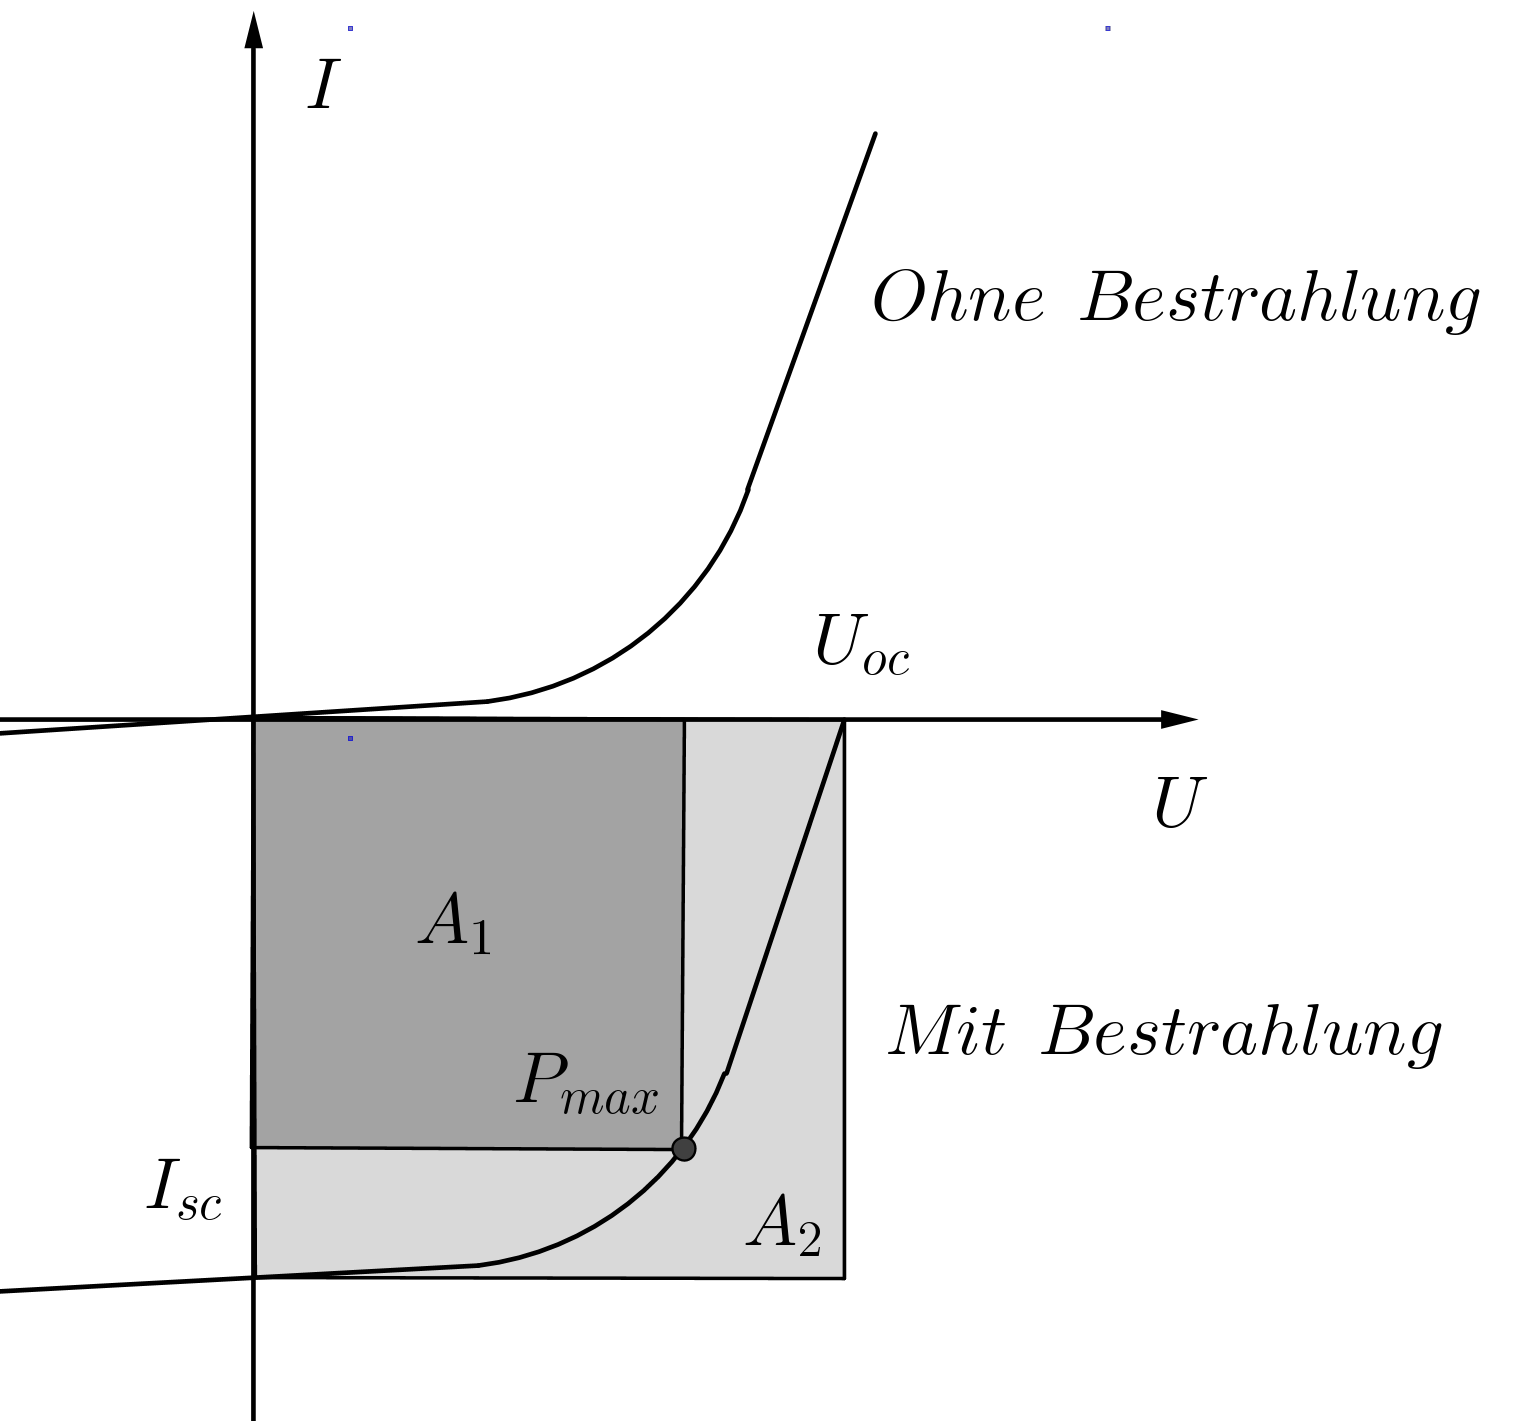
\includegraphics[width=0.5\textwidth]{pics/sol2.png}
\caption{Kennlinie einer Silizium-Solarzelle}
\label{Kennlinie}
\end{figure}

In Abbildung \ref{Kennlinie} schließt die Kennlinie an
diesem Punkt ein Rechteck A$_1$ ein, welches mit dem Rechteck A$_2$ einen Füllfaktor (FF = A$_1$ / A$_2$) ergibt. Der Wirkungsgrad $\eta$
setzt sich aus dem Verhältnis des maximalen Leistung und der eingestrahlten Leistung $P_{\text{ein}}$ zusammen.

\begin{equation}
 \eta = \frac{P_{\text{max}}}{P_{\text{ein}}} = \frac{U_{\text{oc}}\cdot I_{\text{sc}}\cdot \text{FF}}{P_{\text{ein}}}
\end{equation}

\section{Durchführung}
Ziel des Versuchs ist die Ermittlung der Strom-Spannungskennlinien einer Solarzelle für verschiedene Beleuchtungsstärken und daraus
die abgegebene Leistung und der Wirkungsgrad berechnet werden. Darüber hinaus sollen die Leerlaufspannung und der Kurzschlussstrom 
ebenfalls als Funktion der Beleuchtungsstärke bestimmt werden.\\
Hierzu wird die Solarzelle mit einer Lampe verstellbarer Höhe beleuchtet. Die Beleuchtungsstärke nimmt mit zunehmendem Abstand ab. 
Mit zwei Messgeräten werden die anliegende Spannung und der Strom für manuell einstellbare ohmsche Widerstände zwischen 5 und 100 $\Omega$
notiert. 

\section{Auswertung}


\section{Diskussion}

% ========================================
%	Literaturverzeichnis
% ========================================

%\bibliographystyle{plainnat}			% Bibliographie-Style auswählen
%\bibliography{BIBDATEI}			% Literaturverzeichnis

% ========================================
%	Das Dokument endent
% ========================================

\end{document}
